\documentclass[11pt,a4paper]{article}
\title{TFW: Preliminary results for class 150 train, carriage one}
\usepackage{cite}
\usepackage{hyperref}
\usepackage{textcomp}
\usepackage{amssymb}
\usepackage{subcaption}
\usepackage{amsfonts}
\newcommand{\norm}[1]{\left\lVert#1\right\rVert}
\usepackage[left=2cm,right=2cm,top=2cm,bottom=3cm]{geometry}
\usepackage{amsmath}
\setlength\parindent{0pt}
\usepackage{float}
\usepackage{placeins}
\pretolerance=10000
\tolerance=2000
\emergencystretch=10pt
\author{Lucy Henley, Joshua Moore, Timothy Ostler \& Thomas Woolley\footnote{moorej16@cardiff.ac.uk, henleyl1@cardiff.ac.uk, ostlert@cardiff.ac.uk,woolleyt1@cardiff.ac.uk}}
\usepackage{graphicx}
\graphicspath{{./matlab_and_plots/}}
\begin{document}
\maketitle

\section*{Key points}
\begin{itemize}
\item We have run our seat selection code over the old building first floor layout, based on the provided CAD file.
\item We achieved a maximum seat occupancy, with a $2$m social distancing measure, of approximately $45\%$ without shielding, a significant improvement on the benchmark supplied at $28\%$.
\item We have developed a new web-based application which is specific to the Next first floor layout, available \href{https://lucyhenley.shinyapps.io/Next_seating/?fbclid=IwAR2Rx-OmoSkYHlw6BnQSKLgJGQt7VJvaX2IJYbqgKu4MK9YZxoZn1gBBAaEp}{here}. %The code can be found \href{https://github.com/Lucyhenley/Next_app}{here}.
\item We have shown our `greedy algorithm' is sufficient in improving the seating arrangements in Next office buildings.
\end{itemize}

\section*{What we could do next}
\begin{itemize}
\item Given the potential shield locations in the CAD file, we could simulate scenarios using shielding.
\item We can run the code over a greater number of seat choices to try to improve  our solution.
\end{itemize}



\section*{Methods and results}
Following our discussions, we took the CAD file provided and reformatted the information to be compatible with our app. Running the code for one seating order, the results of which are displayed in Figure \ref{Demonstration_pics}.


We initially ran the code under the assumption that the conference rooms could be used. We have also provided the results without the conference rooms included. Results are displayed in Table \ref{tab:performance}.


\begin{figure*}[ht!]
\centering
\begin{subfigure}[h]{0.95\linewidth}
\centering
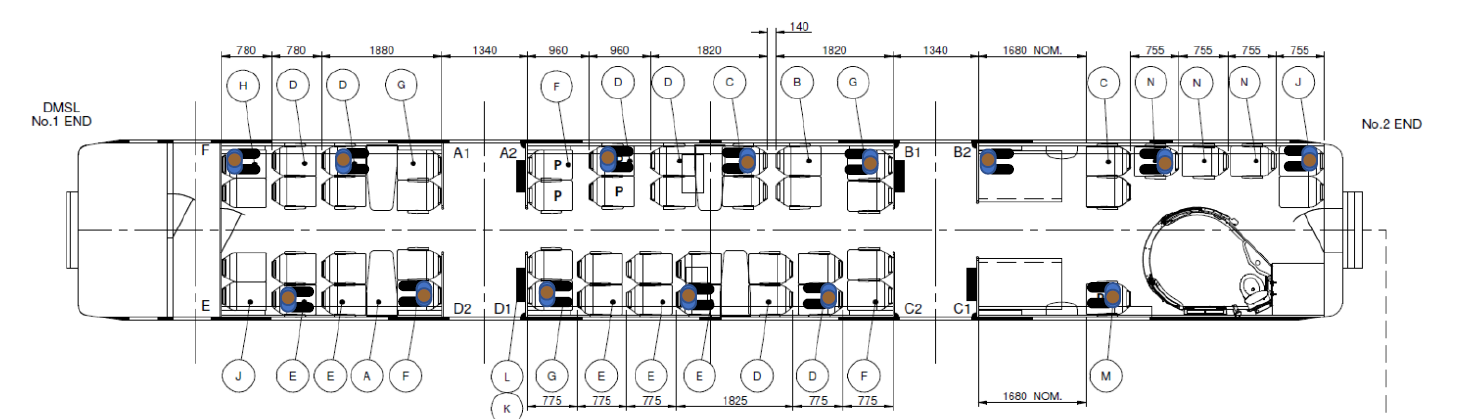
\includegraphics[scale = 0.6]{floorplan150carriage1.png}
\caption{The seating arrangement for the first carriage of a class 150 train.}
\label{Reference}
\end{subfigure}
~
\begin{subfigure}[h]{0.49\linewidth}
\centering
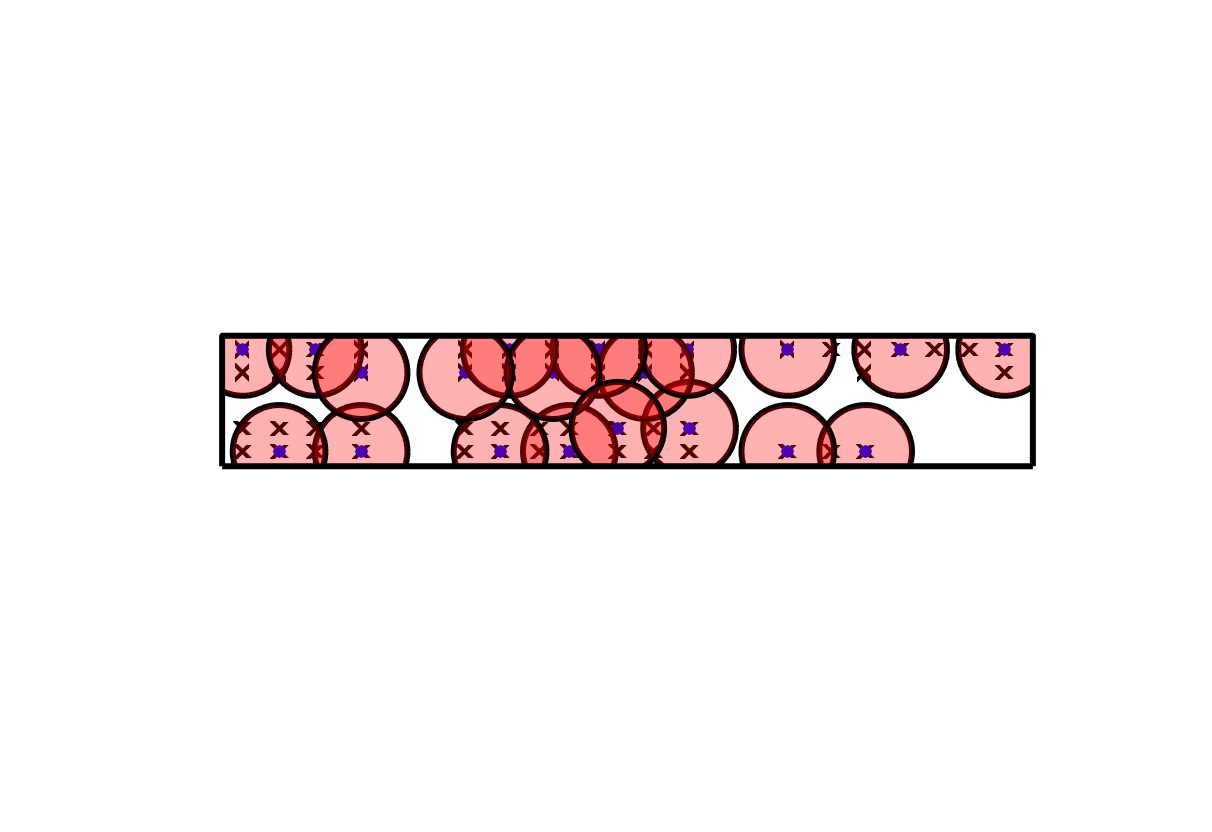
\includegraphics[width = \linewidth]{class150_first_car_1m.png}
\caption{A sample layout for a social distancing measure of $1$ metres, which uses $20$ seats.}
\label{OneMetre}
\end{subfigure}
~
\begin{subfigure}[h]{0.490\linewidth}
\centering
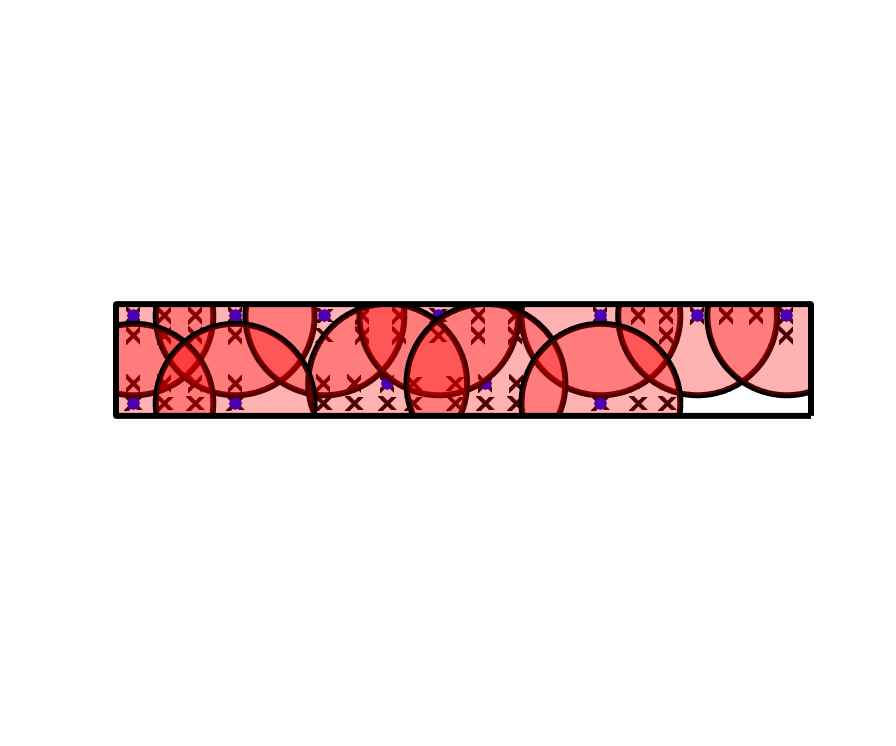
\includegraphics[width = \linewidth]{class150_first_car_2m.png}
\caption{A sample layout for a social distancing measure of $2$ metres, which uses $12$ seats.}
\label{TwoMetre}
\end{subfigure}
\caption{A proposed office layout given by the app for $1$ and $2$ metre social distancing. Seat locations are marked with crosses, available seats are marked with dots and the `region of safety' is denoted by a circle around the available seats. Overlapping circles imply that certain regions are exposed to contamination from multiple sources, but no available seats are located in these regions. }
\label{Demonstration_pics}
\end{figure*}


\begin{table}[ht!]
\begin{center}
 \begin{tabular}{|c |c|}
 \hline
& \textbf{Maximum capacity at $2$m social distancing (\%)}\\
 \hline
 Next CAD file benchmark &   27.9\\
 \hline
 Cardiff App  with conference rooms& 41.5\\
\hline
Cardiff App without conference rooms & 45.2\\
 \hline
\end{tabular}
\end{center}
\caption{Comparison of the performance of the Cardiff seat finding app against the benchmark provided in the supplied CAD file.}
\label{tab:performance}
\end{table}


As demonstrated in Table \ref{tab:performance}, we can very quickly achieve significantly higher occupancy rates in the office without violating social distancing measures. Given more time, we can search for even better solutions, as well as develop methods for user specification of shield locations (see first app).

\section*{Prospective developments for improving optimality}
Our app always provides seating arrangements that obey social distancing measures, and provides locally optimal solutions which are already better than the given benchmarks. Returning the  absolute optimum arrangement, however, is a lot more difficult because the problem is what is known as `NP-hard'.  Simply put, the only way to guarantee you have the most possible seats used is to try every possible order of seat checking, and pick the one which has the most seats used. Actually trying out every seat ordering would take a very long time; there are more ways to order $253$ seats than there are particles in the universe.\\

What we can do, though, is develop techniques to check our solutions and continuously improve upon them where possible. At a cost of additional time and computing power to implement, these methods would improve the likelihood we have found the best possible seating arrangement, allowing us to potentially further improve on our already powerful result.\\

\end{document}
